\documentclass[runningheads]{llncs}
\usepackage{graphicx}
\usepackage{graphicx}
\usepackage{bm}
\usepackage{amsmath}
\usepackage{amssymb}
\usepackage{booktabs}
\usepackage{threeparttable}
\usepackage[ruled]{algorithm2e}
\usepackage{setspace}
\usepackage{float}
\usepackage{caption}
\usepackage{array}
\usepackage{url}
\usepackage{subfigure}


\title{The implementation of a browser-based source code navigator and its cloud solution} % Title
\author{Tong Zhou 180275186}
\institute{School of Computing, Newcastle University \\ Newcastle upon Tyne, NE1 7RU}

\begin{document}
\maketitle

\begin{abstract}
	The blockchain technology, with Bitcoin as its most famous product, is now more and more applied to different industrial areas such as finance, insurance, and smart contract systems. Bitcoin provides a decentralized solution for online cryptocurrencies, and it is claimed that Bitcoin could adequately protect the privacy of the user by using their Bitcoin address instead of IP address\cite{nakamoto2008bitcoin}. But recent researches show that we can still use some modified client with specific algorithms, like Bayesian\cite{juhasz2018bayesian}, to estimate and finally calculate the IP address of a Bitcoin address. Thus, there are still some improvements to be applied to those blockchain systems who want to provide anonymity characteristic to all the participants in their network.
\end{abstract}
%=============================
%=== Introduction ============
%=============================
\section{Introduction}

Bitcoin, as the first decentralized digital currency, is now synonymous of blockchain technology. Back to October in 2008, a paper authored by Satoshi Nakamoto titled Bitcoin: A PeertoPeer Electronic Cash System\cite{nakamoto2008bitcoin} was published and sent to a cryptography mailing list, which was the first time people know the Bitcoin.

After ten years of development, bitcoin has become the most popular cryptocurrency, and there are also a lot of other types of cryptocurrency such as Litecoin, Ripple, Namecoin, etc. Those different cryptocurrencies provide alternative ways for online payment, and some of the technologies have been applied to financial industries such as banking, insurance, and Credit information systems, offering us the possibility of a decentralized and secure way for online financial transaction and information exchange.

In this paper, I give an understandable interpretation to the relationship between Blockchain, Bitcoin and other relevant technologies, and provide a general explanation of how clients in Bitcoin system exchanges with each other. Also, I discuss the anonymity of Bitcoin and introduce a Bayesian Method to get the physical address from the Bitcoin address.


%=============================
%===      Blockchain      ====
%=============================
\section{Blockchain}

Bitcoin itself, designed as a decentralized cryptocurrency, do not rely on any trust third party to fulfilling the entire transaction, which impacts not only cryptocurrency but the whole information technology. But before we discuss its influence, lets firstly have a general idea about the technology bitcoin based on, which is the Blockchain.

As a decentralized data storage technology, Blockchain was firstly described by Satoshi Nakamoto in 2008, as the infrastructure technology of Bitcoin. To begin with, we are going to understand the primary mechanism of the Blockchain.

\subsection{Types of Blockchain}
With the development of blockchain technology, there are several types of different blockchains. According to the network scope, there are three types of blockchains: Public Blockchains, Private Blockchains, and Federated Blockchains.

\subsubsection{Public Blockchains:}
Just like Bitcoin and Litecoin, Public Blockchains provide full access for any user on the internet. There is no authentication to the system users, and all the transactions conducted among the network are available to be retrieved by any of the users.

For example, anyone who want to use Bitcoin just needs to download a client program and create an address for his wallet. Then, he can transit with any other account within Bitcoin network and at the same time view every single transaction that has ever created within the Bitcoin network from back to the first block that was created by Satoshi Nakamoto himself, which is also called Genesis Block. There is no third party can control the network, because every client in the system just works according to the rules defined in the algorithm, these rules must make sure that any honest user in the system can fairly participant the exchange and all fraudulent transactions will finally be recognized and rejected from the system.

Public Blockchains usually used for some system that requires openness and transparency, like online cryptocurrencies and some financial system that open to the public. But it is also apparent that Public Blockchains are exposed to the entire internet. The number of the clients and whether a client is an honest user cannot be promised, so synchronization is always conducted within the system, and only a transaction acknowledged by at least half of the clients can it be regarded as fully accepted by the network.

\subsubsection{Private Blockchains:}
Private Blockchains, just like the opposite concept of Public Blockchains, means a kind of network that only used and accessed internally within a particular scope. Such type of blockchain system usually have some authentication process like register and log in, and may have user role machinimas which control the accessibility of the users.

Within a private blockchain system, the number and the status of the clients and usually within control, so commonly there is no such process like “mining” in a private blockchain. Also, users do not need to compete for mining, so there is no waste on the computing resources for Private Blockchains.

\subsubsection{Federated Blockchains:}
Federated Blockchains is a kind of hybrid system from both Private Blockchains and Public Blockchains; it is commonly used in an environment with multiple roles and users, especially suitable for enterprise affairs that provide certain accessibility to the public but at the same time secure that critical information within the internal network.

\subsection{Mechanism of Blockchain}
Just like the word “Blockchain” itself, blockchain can generally conclude as the combination of “Block” and “Chain”. In a blockchain system, all the data and information stored within a single unit called the Block. Within each block, there are certain numbers of transactions recorded and ordered by time, and these “blocks” distributedly stored in every client that participant in the blockchain system. Every time after a certain period, a new block will be generated with a pointer links to the previous block, which makes all the blocks be connected as a single chain.

\begin{figure}[H]
	\centering
	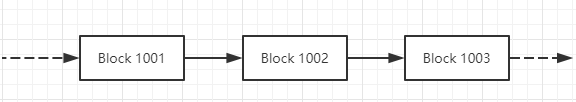
\includegraphics[width=9cm]{reportpics/1.png}
	\caption{Connection of Blocks}
	\label{connection of Blocks}
\end{figure}

Different blockchain system has different periods for generating a new block; for example, Bitcoin takes every 10 minutes\cite{nakamoto2008bitcoin} as a cycle to pack all the transactions in the network.

Looking more detail into every block, each block is consist of two parts: Block Header and Block Transactions.

\begin{itemize}
	\item \textbf{Block Header:} The meta information of every block, with two component:
	      \begin{itemize}
		      \item \textbf{Hash of previous block’s Header;}
		      \item \textbf{Merkle Root of the transactions in the current block.} Which is generally the combinate hash of every single transaction.
	      \end{itemize}
	\item \textbf{Transactions:} A list of transactions that stored within this block.
\end{itemize}

So, a more detailed structure can be drafted like the following diagram.

\begin{figure}[H]
	\centering
	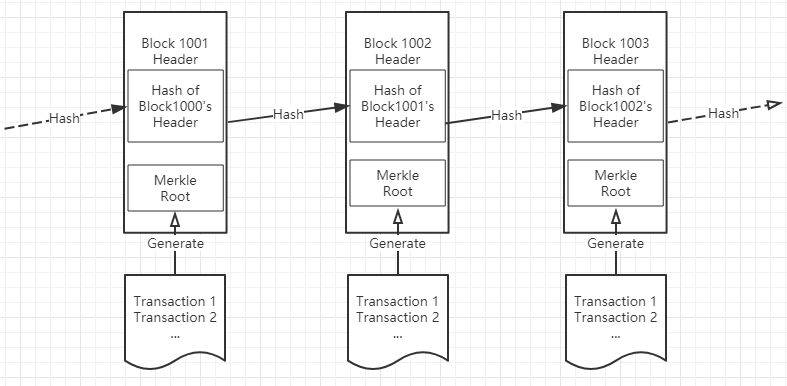
\includegraphics[width=11cm]{reportpics/2.png}
	\caption{Detailed structure of blocks}
	\label{detailed structure of blocks}
\end{figure}

As is shown in the diagram, we use the hash of every transaction to generate the Merkle Root, and we combine the Merkle Root and the hash of previous blocker’s header as the head of current Block.

Within such kind of data structure, for example, if you want to change any transaction within block 1002, you will need to change the Merkle Root in the header of this block, and even worse you will also need to replace all the headers of every following block that connected to this block. Since every client of the blockchain system maintains their own copy of the record, you will have to change half of the clients within the system at least to distort the original recording.

\begin{figure}[H]
	\centering
	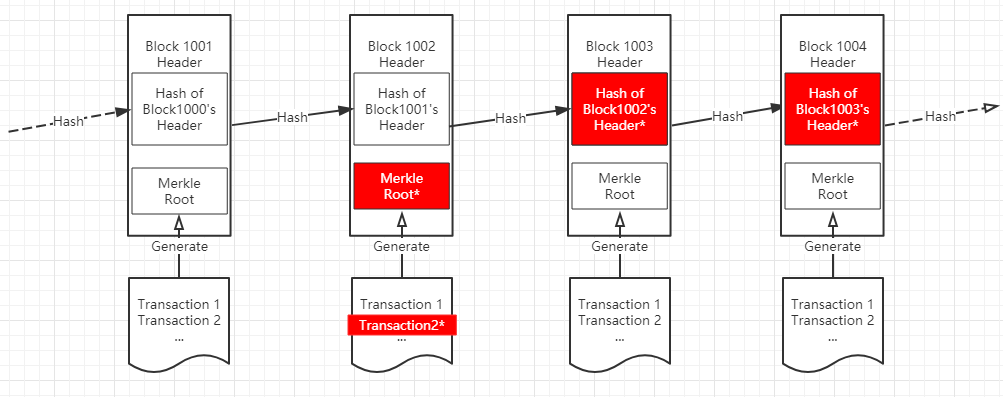
\includegraphics[width=12cm]{reportpics/3.png}
	\caption{How cheated block will influence the other blocks}
	\label{how cheated block will influence the other blocks}
\end{figure}

For those blockchain systems with numerous users, like Bitcoin which have 35 million wallets by 2016\cite{hileman2017global}, it is almost impossible to hack such large amounts of clients in the entire system.

\subsection{Consensus Strategy}

Consensus means some concepts and rules that been accepted and conducted by all the members within a specific group. For traditionally centralized topology, Consensus can be easily distributed and monitored within the system, because every edge nodes(or clients) will only follow the rule required by the centeral node(or server). But as for a decentralized system, there is no such difference like edge and center, client and server within a centralized system, because every client works equally with other clients, and all clients will have to negotiate with other clients to cooperate with each other.

Thus, the consensus strategy is a set of rules that defined how a client within the blockchain system should work with other clients, so within single blockchain system this rule should be unified and obeyed by every working clients.

An essential part that is defined in the blockchain system is the rule of how to select a client to create new blocks. In other words, it is a set of criteria that used to filter out the best client to pack all transactions within a specified period into a new client.

There are several types of solutions to define such kind of criteria:

\subsubsection{PoW (Proof of Work):}

clients are asked to generate some data that is time-consuming and costly, but at the same time easy to validate. Then select the client that firstly gets this validated data as the winner, so that to prove that this client has enough capacity for generating a new block for the entire network. This is the solution adopted by the Bitcoin System. However, PoW actually takes a lot of capacity to calculate the target data, and it is a waste of resources for so many computers to generate useless random data.

\subsubsection{PoS (Proof of Stake):}

Different from PoW, PoS uses a pseudo-random algorithm to select clients from all candidates with different proportions, which related to the amount of the coin this client has. The word “Stake” in PoS means how much fortune a client has. In other words, those clients with more coins will be more likely to be selected.

PoS is designed to reduce the waste of resource in PoW and is used by some new cryptocurrency like PeerCoin\cite{peercoin} and BlackCoin\cite{blackcoin}.

\subsubsection{DPoS (Delegate Proof of Stake):}

With DPoS solution, all clients within the blockchain network are classified into two types: Normal Users and Delegates. Delegates is a type of users that are voted by Normal Users; all these Delegates works equally with each other and responsible for validating the transactions within the network, packing these transactions into new clients and then broadcast these clients.

\subsubsection{PBFT (Practical Byzantine Fault Tolerance):}

PBFT solution is a more complicated way for consensus strategy in a blockchain system. In the PBFT algorithm, it pointed out that when there are n clients altogether in the network and f clients out of them are dishonest or damaged clients, only when:

\begin{equation}
	3f+1<=n\label{equ:pbftInequality}
\end{equation}
Equation (\ref{equ:pbftInequality}) is the inequality for PBFT algorithmo\cite{castro1999practical}.

\begin{equation}
	\therefore f<= (n-1)/3
\end{equation}


Then the network can eliminate the Impact of dishonest clients. At the same time, the complexity of the algorithm is:

\begin{equation}
	o(n^2)\label{equ:pbftComplexity}
\end{equation}
Equation (\ref{equ:pbftComplexity}) is the complexity for PBFT algorithmo\cite{castro1999practical}.

~\\
There are four steps for a full PBFT process:

\begin{enumerate}
	\item The client sends a request to the main stub;
	\item The main stub broadcast the request to other stubs, and those stubs execute the PBFT 3-phase process;
	\item After the stubs finish the process, return a message to the client;
	\item After the client receives the same messages from f+1 clients, the PBFT process is regarded as completed successfully.
\end{enumerate}

As you may find in the PBFT algorithm, there is a role of “main stub” within the entire lifecycle, which means this kind of consensus strategy cannot be used for any public blockchains. In fact, PBFT is commonly used for Federated Blockchains, which provides a high ability of fault tolerance to the entire network within the system.

There are also some other kinds of consensus strategy, but these four solutions listed above are the most popular ones that are generally used in blockchain systems.

%=============================
%=== Mechanisms of Bitcoin====
%=============================

\section{Mechanisms of Bitcoin}
After we got some general idea about blockchain, we can now more detailly talk about Bitcoin itself. Firstly we are going to understand how Bitcoin clients are connected and work with each other clients (nodes).

\subsection{The Bitcoin network}
Traditional structure for a C/S online system is usually a centralized star topology, which means all client nodes are connected to one or more central nodes, and these client nodes have no direct connection between each other, which simplify the complexity of the network.


For example, when you use PayPal to pay 20 pounds to your friend, you first connect to the central server provided by PayPal, and then PayPal server process the request. Finally, it sends a message to your friend about this transaction.

\begin{figure}[htbp]
	\centering
	\begin{minipage}[t]{0.53\textwidth}
		\centering
		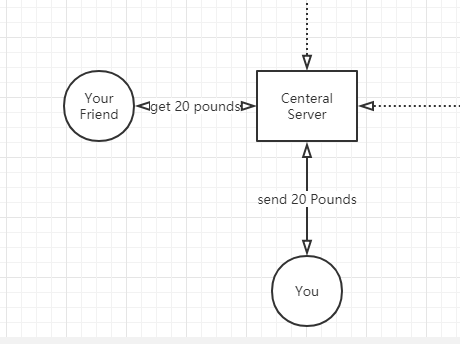
\includegraphics[height=4cm]{reportpics/4.png}
		\caption{Traditional centralized topology}
	\end{minipage}
	\begin{minipage}[t]{0.42\textwidth}
		\centering
		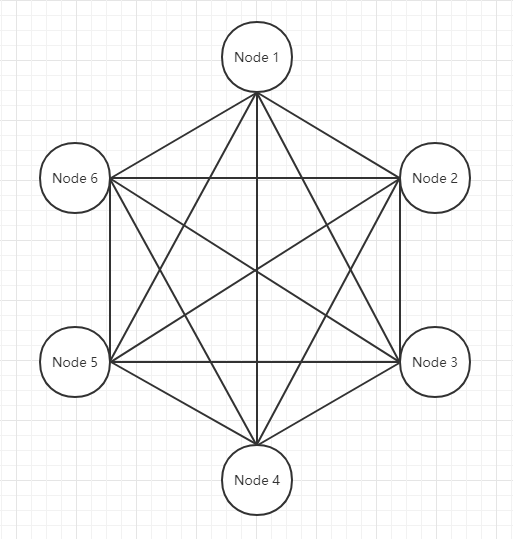
\includegraphics[height=4cm]{reportpics/5.png}
		\caption{Fully connected topology in decentralized system}
	\end{minipage}
\end{figure}

But it is not feasible for peer-to-peer systems like Bitcoin. In the Bitcoin network, every single running clients are trying to connect other reachable clients. Although there are different types of bitcoin application with various functions and physical location, however within one blockchain network they still share the same consensus strategy that defined how these clients cooperate with each other.

Before every client starts to synchronize transactions, there is a message protocol that explores all reachable clients within the network\cite{asharaf2017decentralized}. The general process can be described with the following steps:

\begin{enumerate}
	\item The client starts the message protocol, and connect all the clients that already known by this client with authorized information to establish a connection;
	\item When connection found, send them a list of neighbors that stored in current client to another client, and get the neighbor list that provides by the other client;
	\item If the current client has not connected the new neighbor, then try to connect this new client. If connected successfully, save this client into local neighbor list;
	\item If there is no any reachable neighbor, try to find new neighbors on the internet, and save them to a neighbor list if successfully connected.
\end{enumerate}

\subsection{Bitcoin wallet}

The Bitcoin wallet is a kind of front-end component that directly operated by the end user. It is used to create and inquiry transactions. Also it can help the user to manage Bitcoin addresses. There are two kinds of Bitcoin wallet the in terms of the information it synchronizes Core Wallet and Lightning Wallet.


\begin{itemize}
	\item \textbf{Core Wallet:} A comprehensive type wallet that contains all the transactions from the first day Bitcoin is published. There are more than 400GBs of transaction data till 21. March 2019, and it takes about 20 hours to synchronize the transaction for the first time we use the core wallet. 
	\item \textbf{Lightning Wallet: } Also called SPV wallet (Simplified Payment Verification). SPV wallet only downloads all the header message of ever blocks, which is much less than the entire block with all transactions, and it uses the Merkle Root of the header to validate any transaction. 
\end{itemize}

Apparently, SPV wallet is more convenient that Core Wallet, but as a compromise, it sacrificed the safety to support a much portable client that can even installed in mobile devices.


\subsection{Proof-of-work and Bitcoin Mining}

The Bitcoin system use PoW solution to select which node(client) is authorized to pack all the transactions within a specified period (about every 10 minutes\cite{nakamoto2008bitcoin} in Bitcoin Network). The mechanism of PoW has been explained in section 2.3, but why these users are chased to spend so many resources to compete for the right to pack the transactions?

We already know that Bitcoin is a kind of decentralized peer-to-peer network, which means every client maintains their own copy of transactions, and there is no some central server that works as an authorized data source for another client to synchronize. So to keep the consistency of all the data between different clients, the system will select some specific clients to pack all the transactions within this period, and then get extra bitcoins from the system as the reward of its work. This process is also the way that Bitcoin issues new coins into the market.

There are four steps for Mining process:
\begin{enumerate}
	\item \textbf{Compete for packing:} Every client that participant in mining will compete for packing by PoW, whoever calculate the result first will be selected to pack the new block;
	\item \textbf{Validate transactions:} The selected client will validate all the transaction it received and then pack them into a new block;
	\item \textbf{Earn and issue extra coins:} In the transaction list of the block there will be a new transaction that indicates that some bitcoins are issued and given to the address of this client as a return of its work;
	\item \textbf{Broadcast the new block:} This client will then broadcast this new block to all his neighbor, other clients will validate the new block and then broadcast to other neighbors.
\end{enumerate}

After these steps, a new block will be created and the miner will start to compete for new blocks.

%=============================
%===      Anonymity       ====
%=============================

\section{Anonymity}

\subsection{The anonymity of the Bitcoin and the Sociology impact}

According to what described in Bitcoin White Paper,  the privacy of Bitcoin transaction can be ensured by using the Bitcoin address instead of the IP address during the exchange. Users can even hold multiple Bitcoin addresses and use different addresses for every single transaction to keep the privacy\cite{nakamoto2008bitcoin}. 

Although anonymity is not the primary purpose for Bitcoin, it is still widely identified that Bitcoin is a kind of online cryptocurrency with high-level anonymity. 

Bitcoin and other Blockchain technologies even have a lot of implications to international money laundering due to two specific features: the decentralization and quasi-anonymity of transactions on global networks\cite{campbell2017bitcoin}. 

\subsection{Tracking transactions in the Bitcoin network}

But in fact, as a public blockchain, every single transaction within the Bitcoin network can be tracked as long as you have the Bitcoin address either from sender or receiver. Which means, if you can trace any Bitcoin address that belongs to some specific user, then all the other addresses that ever have transactions with this Bitcoin address can be easily recognized.

Moreover, merely getting revealed of all Bitcoin address is not even the worst situation. It is also possible for an attacker to retrieve your real IP address according to the Bitcoin address you use with the help of only hundreds of modified Bitcoin Client application\cite{juhasz2018bayesian}.

\subsection{Two steps for user identification}

Before we start to identify the user, we will have some modified Bitcoin client that injected with some predefined codes to observe the entire Bitcoin network, which is called monitoring clients. Since Bitcoin is an opensource project, we can easily adjust the source code of the Bitcoin Client. 

Then the monitoring client will start to record the IP address of the neighbors that directly connected to it. After we have hundreds of monitoring clients within the entire bitcoin network, we can collect a lot of datasets with the tip of a client and the transactions it passed to your client.


\subsection{Assign probabilities with Bayesian Method}

Bayesian probability is a kind of explanation to the concept of probability which is interpreted as reasonable expectation\cite{cox1946probability} or representing a state of knowledge\cite{jaynes1986bayesian}. In this section, the Bayesian method is used to calculate the probability. There are two main steps to identify the users within a running Bitcoin network:

\begin{enumerate}
	\item Determine the probability of each transaction that is created by a specific client with IP address information fetched by monitoring clients. Within step 1 there may already generate some possible IP-address – Bitcoin pairings;
	\item By grouping the Bitcoin address from an identical user that have high probability on a transaction network, the most likely pairings will be identified from the previous step.
\end{enumerate}

Finally, the geographical location can easily be queried with the IP address acquired with these two steps.

More detailed calculus process is explained in the research of A Bayesian Approach to Identify Bitcoin Users\cite{juhasz2018bayesian} which gives all the equation that is used. But this way is just like a random retrieving from the entire Bitcoin network, you do can find some IP address from specific client, but it is too difficult to get the IP address from any single Bitcoin address.

But still, we can find that the anonymity is not sufficiently assured within current Bitcoin network, and further solutions remain to be designed to keep the privacy of Bitcoin transactions.

\section{Conclusion}
After decades of research and practice, Blockchain technology is now more and more optimized and well improved. Different kind of Blockchain systems like Ethereum and HyperLedger provide with many integrated development tools so that users can quickly build their own Blockchain system.

On the other hand, the privacy of the user not adequately secured by the Bitcoin system; a potential attacker can still get geography information from some of the clients by mathematical methods like Bayesian.

Although there is some potential issue within blockchain products like Bitcoin, it remains to be the most popular online cryptocurrency. In the future, we will need to improve both the Legal System and the technology of blockchain to make it contribute to our society better.


\newpage
\bibliographystyle{plain}
\bibliography{reference}

\end{document}